\documentclass[tikz,border=0pt]{standalone}
\usepackage{xcolor}
\usetikzlibrary{calc}
% Palette: Sam_Comm_final.png by eye, and the drones and raiders.
\definecolor{ink}{HTML}{3B2340}
\definecolor{sky}{HTML}{EFC46A}
\definecolor{skyhi}{HTML}{F5DA92}
\definecolor{skylow}{HTML}{E9B060}
\definecolor{cloud}{HTML}{F2D58A}
\definecolor{paper}{HTML}{FBEFD0}
\definecolor{cream}{HTML}{FFF6E0}
\definecolor{white}{HTML}{FFFFFF}
\definecolor{wallA}{HTML}{E88A73}
\definecolor{wallB}{HTML}{EE9F7E}
\definecolor{wallC}{HTML}{E47A7E}
\definecolor{wallD}{HTML}{F0B07E}
\definecolor{wallE}{HTML}{D9765F}
\definecolor{wallF}{HTML}{E99A8A}
\definecolor{greenA}{HTML}{8DBB7E}
\definecolor{greenB}{HTML}{6FA77A}
\definecolor{greenC}{HTML}{A9C97F}
\definecolor{greenD}{HTML}{5E9C6A}
\definecolor{greenE}{HTML}{4A8060}
\definecolor{sage}{HTML}{9DB98A}
\definecolor{sagedark}{HTML}{6F8F66}
\definecolor{sagelight}{HTML}{C2D6A6}
\definecolor{window}{HTML}{F6E7A0}
\definecolor{windark}{HTML}{8C5A64}
\definecolor{metal}{HTML}{8D9A93}
\definecolor{metaldark}{HTML}{5E6B66}
\definecolor{metallight}{HTML}{B9C4BC}
\definecolor{wood}{HTML}{B9835A}
\definecolor{wooddark}{HTML}{8C5A3C}
\definecolor{woodlight}{HTML}{D9A66F}
\definecolor{stone}{HTML}{E7C9A0}
\definecolor{stonedark}{HTML}{C9A47E}
\definecolor{concrete}{HTML}{D8C3A4}
\definecolor{concretedark}{HTML}{B8A084}
\definecolor{asphalt}{HTML}{8E7A86}
\definecolor{asphaltdark}{HTML}{6E5C68}
\definecolor{roadline}{HTML}{F6E7A0}
\definecolor{kerb}{HTML}{D8B48C}
\definecolor{red}{HTML}{E0483E}
\definecolor{redlight}{HTML}{F27A6A}
\definecolor{gold}{HTML}{FFB000}
\definecolor{goldlight}{HTML}{FFD54F}
\definecolor{teal}{HTML}{4FA3A0}
\definecolor{tealdark}{HTML}{3C8582}
\definecolor{magenta}{HTML}{FF2E88}
\definecolor{cyan}{HTML}{13CFE3}
\definecolor{violet}{HTML}{8A5BD6}
\definecolor{orange}{HTML}{F2803A}
\definecolor{pink}{HTML}{F48FB1}
\definecolor{glow}{HTML}{4FE6E0}
\definecolor{glowhi}{HTML}{C8FFF9}
\definecolor{hot}{HTML}{FF6A1A}
\definecolor{hothi}{HTML}{FFD07A}
\definecolor{armour}{HTML}{7E7A86}
\definecolor{armourdark}{HTML}{5A5466}
\definecolor{armourlight}{HTML}{A8A2B0}
\definecolor{wasp}{HTML}{E0A82E}
\definecolor{waspdark}{HTML}{B07E1A}
\definecolor{moth}{HTML}{F2E6C8}
\definecolor{mothdark}{HTML}{D2C09A}
\definecolor{hornet}{HTML}{3C8582}
\definecolor{hornetdark}{HTML}{2C6260}
\definecolor{warden}{HTML}{E47A7E}
\definecolor{wardendark}{HTML}{B85A62}
\definecolor{tick}{HTML}{8DBB7E}
\definecolor{tickdark}{HTML}{5E8A5A}
\definecolor{strider}{HTML}{D9765F}
\definecolor{striderdark}{HTML}{A8543F}
\definecolor{jacket}{HTML}{6FA77A}
\definecolor{jacketb}{HTML}{4FA3A0}
\definecolor{jacketc}{HTML}{E88A73}
\definecolor{jacketd}{HTML}{F0B07E}
\definecolor{skin}{HTML}{F2C49A}
\definecolor{skinb}{HTML}{C98C6A}
\definecolor{skinc}{HTML}{8C5A3C}
\definecolor{hair}{HTML}{3B2340}
\definecolor{goo}{HTML}{B6E35A}
\definecolor{goodark}{HTML}{7FB23A}
\newcommand{\Ink}{1.6pt}
\tikzset{inked/.style={draw=ink, line width=\Ink, line join=round, line cap=round}}
\begin{document}
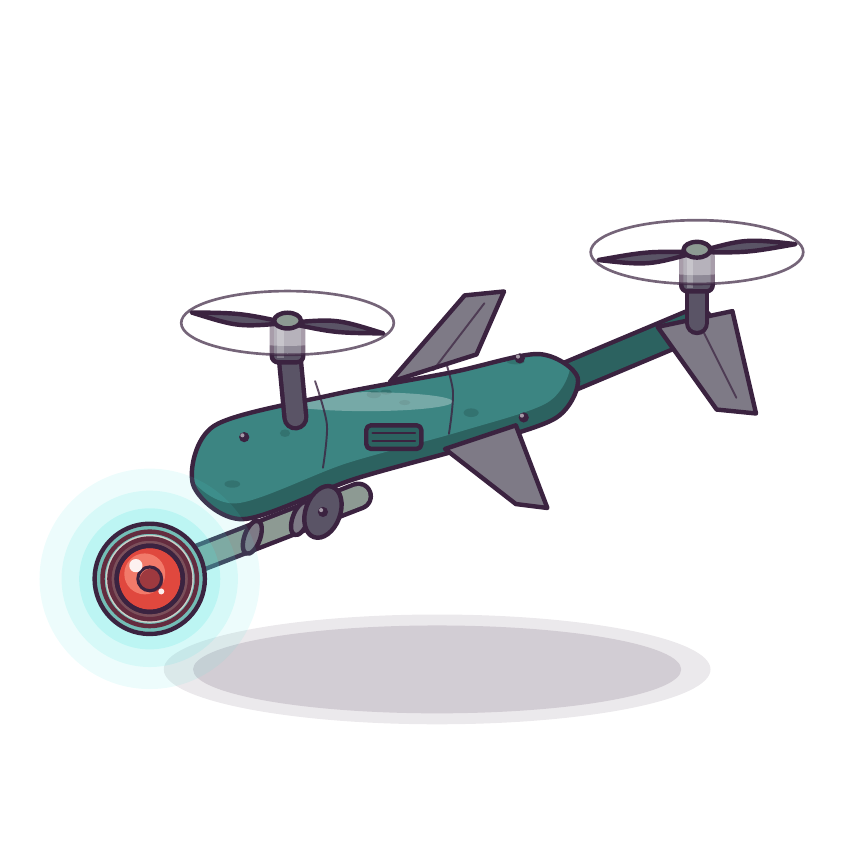
\begin{tikzpicture}
\clip (0,0) rectangle (10,10);
\begin{scope}[shift={(0,-0.35)}, scale=1]
\fill[ink, opacity=0.10] (5.2,2.2) ellipse (3.472 and 0.697);
\fill[ink, opacity=0.14] (5.2,2.2) ellipse (3.1 and 0.558);
\draw[ink, line width=12.305pt, line cap=round, line join=round] plot[smooth, tension=0.55] coordinates {(6,5.55) (8.5,6.6)};
\draw[hornetdark, line width=9.105pt, line cap=round, line join=round] plot[smooth, tension=0.55] coordinates {(6,5.55) (8.5,6.6)};
\filldraw[inked,fill=armour] (8,6.55) -- (8.95,6.75) -- (9.25,5.45) -- (8.75,5.5) -- cycle;
\draw[ink, line width=0.7pt, line cap=round,opacity=0.7] (8.55,6.55) -- (9,5.65);
\draw[ink, line width=8.891pt, line cap=round, line join=round] plot[smooth, tension=0.55] coordinates {(8.5,6.6) (8.5,7.35)};
\draw[armourdark, line width=5.691pt, line cap=round, line join=round] plot[smooth, tension=0.55] coordinates {(8.5,6.6) (8.5,7.35)};
\filldraw[inked,fill=armourdark,rounded corners=0.08cm] (8.3,7) rectangle (8.7,7.52);
\fill[white, opacity=0.25] (8.37,7.05) rectangle (8.45,7.46);
\filldraw[ink, line width=0.96pt, fill=white, fill opacity=0.32, draw opacity=0.7] (8.5,7.5) ellipse (1.35 and 0.405);
\fill[white, opacity=0.35] (8.5,7.5) ellipse (0.972 and 0.292);
\filldraw[inked,fill=armourdark] (8.5,7.5) .. controls (9.116,7.67) .. (9.752,7.601) .. controls (9.131,7.491) .. (8.5,7.5) -- cycle;
\filldraw[inked,fill=armourdark] (8.5,7.5) .. controls (7.884,7.33) .. (7.248,7.399) .. controls (7.869,7.509) .. (8.5,7.5) -- cycle;
\filldraw[inked,fill=metal] (8.5,7.53) ellipse (0.17 and 0.1);
\draw[ink, line width=10.598pt, line cap=round, line join=round] plot[smooth, tension=0.55] coordinates {(4.2,4.4) (1.75,3.45)};
\draw[metal, line width=7.398pt, line cap=round, line join=round] plot[smooth, tension=0.55] coordinates {(4.2,4.4) (1.75,3.45)};
\filldraw[inked,fill=armour,rotate around={-20:(3.465,4.115)}] (3.465,4.115) ellipse (0.1 and 0.22);
\filldraw[inked,fill=armour,rotate around={-20:(2.853,3.878)}] (2.853,3.878) ellipse (0.1 and 0.22);
\fill[hornetdark] plot[smooth cycle, tension=0.5] coordinates {(2.366,5.292) (3.855,5.684) (5.382,5.972) (6.489,6.205) (6.985,5.905) (6.711,5.395) (5.618,5.028) (4.145,4.616) (2.734,4.108) (2.1,4.55)};
\begin{scope}\clip plot[smooth cycle, tension=0.5] coordinates {(2.366,5.292) (3.855,5.684) (5.382,5.972) (6.489,6.205) (6.985,5.905) (6.711,5.395) (5.618,5.028) (4.145,4.616) (2.734,4.108) (2.1,4.55)};
\begin{scope}[shift={(-0.1,0.2)}]\fill[hornet] plot[smooth cycle, tension=0.5] coordinates {(2.366,5.292) (3.855,5.684) (5.382,5.972) (6.489,6.205) (6.985,5.905) (6.711,5.395) (5.618,5.028) (4.145,4.616) (2.734,4.108) (2.1,4.55)};\end{scope}
\begin{scope}\clip plot[smooth cycle, tension=0.5] coordinates {(2.366,5.292) (3.855,5.684) (5.382,5.972) (6.489,6.205) (6.985,5.905) (6.711,5.395) (5.618,5.028) (4.145,4.616) (2.734,4.108) (2.1,4.55)};
\fill[hornetdark, opacity=0.5] (6.199,6.107) ellipse (0.112 and 0.033);
\fill[hornetdark, opacity=0.5] (4.868,5.163) ellipse (0.087 and 0.035);
\fill[hornetdark, opacity=0.5] (3.268,5.2) ellipse (0.065 and 0.048);
\fill[hornetdark, opacity=0.5] (2.599,4.554) ellipse (0.1 and 0.047);
\fill[hornetdark, opacity=0.5] (4.551,5.722) ellipse (0.075 and 0.032);
\fill[hornetdark, opacity=0.5] (5.632,5.46) ellipse (0.096 and 0.055);
\fill[hornetdark, opacity=0.5] (6.383,5.053) ellipse (0.103 and 0.045);
\fill[hornetdark, opacity=0.5] (4.788,5.589) ellipse (0.072 and 0.033);
\fill[hornetdark, opacity=0.5] (4.396,5.692) ellipse (0.091 and 0.048);
\fill[hornetdark, opacity=0.5] (5.07,4.728) ellipse (0.062 and 0.043);
\end{scope}
\fill[white, opacity=0.3] (4.3,5.6) ellipse (1.1 and 0.12);
\end{scope}
\draw[inked] plot[smooth cycle, tension=0.5] coordinates {(2.366,5.292) (3.855,5.684) (5.382,5.972) (6.489,6.205) (6.985,5.905) (6.711,5.395) (5.618,5.028) (4.145,4.616) (2.734,4.108) (2.1,4.55)};
\draw[ink, line width=0.7pt, line cap=round, line join=round, opacity=0.8] plot[smooth, tension=0.5] coordinates {(3.65,5.861) (3.8,5.311) (3.75,4.761)};
\draw[ink, line width=0.7pt, line cap=round, line join=round, opacity=0.8] plot[smooth, tension=0.5] coordinates {(5.25,6.292) (5.4,5.742) (5.35,5.192)};
\filldraw[inked,fill=hornetdark,rounded corners=0.06cm] (4.3,5) rectangle (5,5.3);
\draw[ink, line width=0.8pt, line cap=round] (4.38,5.1) -- (4.92,5.1);
\draw[ink, line width=0.8pt, line cap=round] (4.38,5.2) -- (4.92,5.2);
\fill[ink] (2.75,5.15) circle (0.065);
\fill[white, opacity=0.55] (2.727,5.173) circle (0.026);
\fill[ink] (6.25,6.15) circle (0.065);
\fill[white, opacity=0.55] (6.227,6.173) circle (0.026);
\fill[ink] (6.3,5.4) circle (0.065);
\fill[white, opacity=0.55] (6.277,5.423) circle (0.026);
\filldraw[inked,fill=armour] (4.6,5.85) -- (5.7,6.2) -- (6.05,7) -- (5.55,6.95) -- cycle;
\filldraw[inked,fill=armour] (5.3,5) -- (6.2,5.3) -- (6.6,4.25) -- (6.2,4.3) -- cycle;
\draw[ink, line width=0.7pt, line cap=round,opacity=0.7] (5.15,6) -- (5.8,6.85);
\draw[ink, line width=9.46pt, line cap=round, line join=round] plot[smooth, tension=0.55] coordinates {(3.4,5.4) (3.3,6.45)};
\draw[armourdark, line width=6.26pt, line cap=round, line join=round] plot[smooth, tension=0.55] coordinates {(3.4,5.4) (3.3,6.45)};
\filldraw[inked,fill=armourdark,rounded corners=0.08cm] (3.1,6.1) rectangle (3.5,6.62);
\fill[white, opacity=0.25] (3.17,6.15) rectangle (3.25,6.56);
\filldraw[ink, line width=0.96pt, fill=white, fill opacity=0.32, draw opacity=0.7] (3.3,6.6) ellipse (1.35 and 0.405);
\fill[white, opacity=0.35] (3.3,6.6) ellipse (0.972 and 0.292);
\filldraw[inked,fill=armourdark] (3.3,6.6) .. controls (3.922,6.653) .. (4.518,6.467) .. controls (3.902,6.474) .. (3.3,6.6) -- cycle;
\filldraw[inked,fill=armourdark] (3.3,6.6) .. controls (2.678,6.547) .. (2.082,6.733) .. controls (2.698,6.726) .. (3.3,6.6) -- cycle;
\filldraw[inked,fill=metal] (3.3,6.63) ellipse (0.17 and 0.1);
\filldraw[inked,fill=armourdark,rotate around={-20:(3.75,4.2)}] (3.75,4.2) ellipse (0.22 and 0.34);
\fill[ink] (3.75,4.2) circle (0.065);
\fill[white, opacity=0.55] (3.727,4.223) circle (0.026);
\fill[glow, opacity=0.1] (1.55,3.35) ellipse (1.4 and 1.4);
\fill[glow, opacity=0.14] (1.55,3.35) ellipse (1.12 and 1.12);
\fill[glow, opacity=0.2] (1.55,3.35) ellipse (0.896 and 0.896);
\filldraw[inked,fill=glow] (1.55,3.35) ellipse (0.7 and 0.7);
\fill[glowhi]  (1.466,3.434) ellipse (0.385 and 0.385);
\fill[white, opacity=0.9] (1.27,3.63) circle (0.126);
\filldraw[inked,fill=glow] (1.55,3.35) circle (0.6);
\draw[glowhi, line width=1.6pt] (1.55,3.35) circle (0.53);
\filldraw[inked,fill=armourdark] (1.55,3.35) circle (0.512);
\fill[red, opacity=0.25] (1.55,3.35) circle (0.672);
\filldraw[inked,fill=red] (1.55,3.35) circle (0.42);
\fill[redlight] (1.487,3.413) circle (0.26);
\fill[red!60!ink] (1.571,3.329) circle (0.151);
\draw[ink, line width=1.12pt] (1.55,3.35) circle (0.151);
\fill[white, opacity=0.9] (1.374,3.518) circle (0.084);
\fill[white, opacity=0.9] (1.697,3.19) circle (0.038);
\draw[inked] (1.55,3.35) circle (0.42);
\end{scope}
\end{tikzpicture}
\end{document}
